% !TeX spellcheck = cs_CZ
% !TeX program = pdflatex
\documentclass[10pt,a4paper]{article}
\usepackage[czech]{babel}
\usepackage{cvstyle}

\begin{document}

\begin{sidebar}
{\Large Petr \textsc{Šimčák}}\par\vspace*{0.4ex}
{\small Tech Lead \& softwarový vývojář}\par\vspace*{1.8ex}

\centering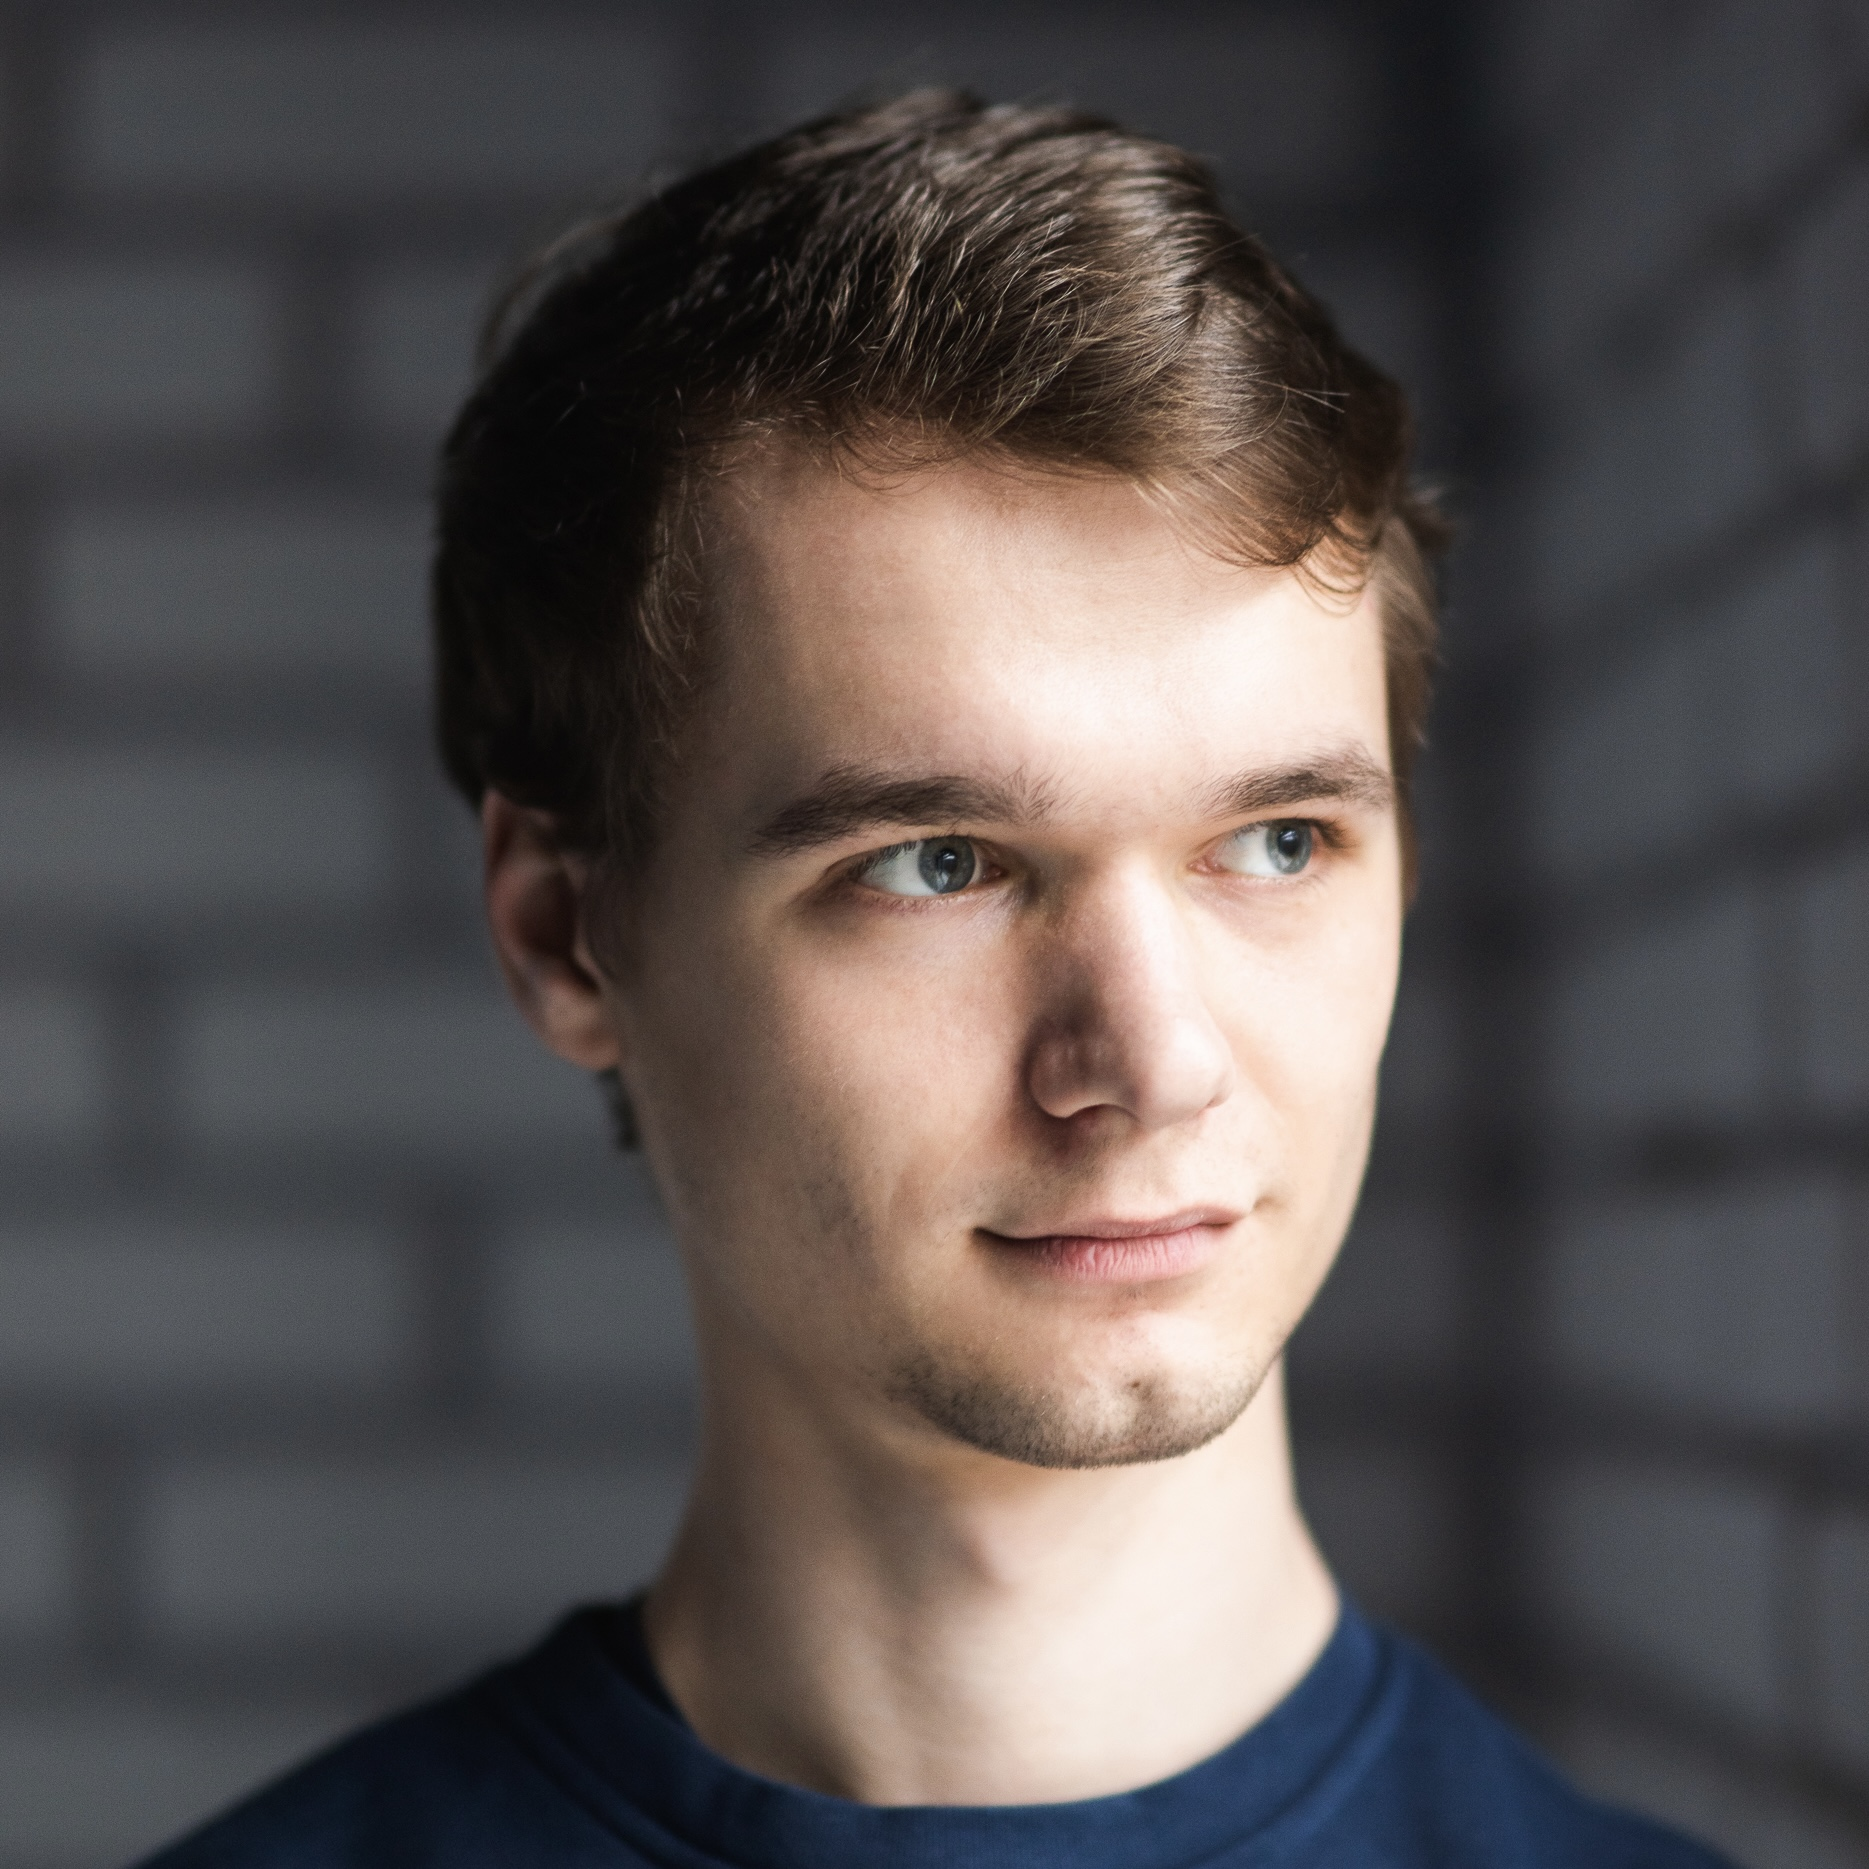
\includegraphics[width=0.8\textwidth]{me.jpg}\par
\raggedright

\sidehead{Profil}
Tech Lead v~AI Campu a~softwarový vývojář, který se k~technologiím dostal od divadla a~filmu.
Zajímá mě, jak AI mění práci lidí a~fungování organizací.
Hledám rovnováhu mezi rychlostí a~kvalitou. Efektivitu, která neobětuje výsledek.
Spojuji technické myšlení s~komunikací a~vystupováním a~nejvíc mě baví měnit nápady ve fungující věci.

\sidehead{Kontakt}
{\small
\contact{\faEnvelope}{\href{mailto:peta.simcak@gmail.com}{peta.simcak@gmail.com}}
\makebox[1.5em][l]{\faLinkedin}\href{https://www.linkedin.com/in/petr-simcak}{linkedin.com/in/petr-simcak}\par}
\contact{\faPhone}{+420\,601\,381\,619}
\contact{\faGlobe}{\href{https://simcak.github.io}{simcak.github.io}}

\sidehead{Dovednosti}
{\small
\begin{itemize}
\item Praktické využití LLM a~AI nástrojů, výuka AI pro firmy
\item C, C++, Python, JavaScript, Shell, SQL, MATLAB
\item Git, Docker, Linux, Nginx, LaTeX
\item Backend, frontend, systémové a~síťové programování
\item Zpracování a~analýza signálů
\end{itemize}}

\sidehead{Jazyky}
{\small
Čeština (rodilý mluvčí) \\[0.4ex]
Angličtina (C1) \\[0.4ex]
Němčina (B1)\par}

\sidehead{Ocenění a~další}
{\small
\begin{itemize}
\item 1.~místo v~kategorii Education Platform, Greenhack (2026)
\item 3.~místo, Škoda Hackathon (2025)
\item 2.~místo, Škoda Hackathon (2024)
\item Cena pro nejlepšího mladého herce, Zlín Film Festival (2014)
\end{itemize}}
\end{sidebar}%
\begin{maincolumn}

\mainhead{Pracovní zkušenosti}

\cventry{Tech Lead}{AI Camp}{2026 -- současnost}{%
\begin{itemize}
\item Lektoruji a~podporuji klienty z~velkých firem v~efektivním a~kreativním využívání LLM a~dalších AI technologií.
\item Zodpovídám za údržbu a~vývoj vzdělávacího programu a~interních nástrojů AI Campu.
\end{itemize}}

\cventry{Softwarový vývojář}{Moneco, skupina Broker Consulting}{2026}{%
Navrhl jsem a~vyvinul OK-Form, hlasovací a~prioritizační aplikaci pro investiční výbor, která nahradila Google Forms. Funguje bez serveru, databáze i~měsíčních poplatků: statický web na GitHub Pages, sběr lístků e-mailem a~automatické zpracování výsledků do CSV a~Excelu přes GitHub Actions a~Python. \href{https://github.com/custom-alg/OK-Form}{GitHub}}

\cventry{Hitchhiker}{42 Prague}{2026 -- současnost}{%
Reprezentuji školu a~její hodnoty na akcích, pomáhám novým studentům a~přebírám zodpovědnost za férový průběh studia ostatních.}

\cventry{Správa 3D tiskáren}{VUT v~Brně, 42 Prague}{2022 -- současnost}{%
Sestavil jsem 3D tiskárnu na VUT a~později zajišťoval provoz, údržbu a~podporu 3D~tiskáren na 42~Prague.}

\cventry{Filmový herec}{české, německé a~americké produkce}{2013 -- 2021}{%
Role ve filmech a~seriálech v~několika jazycích, hlavní role ve filmu \uv{Pojedeme k~moři} (2014). Dlouhodobá spolupráce v~náročných produkcích, práce pod tlakem a~disciplína. \href{https://www.imdb.com/name/nm5791331/}{IMDb}}

\cventry{Divadelní herec}{Městské divadlo Brno}{2009 -- 2015}{%
Sedm inscenací od osmi let, včetně jedné z~hlavních rolí v~muzikálu Mary Poppins. \href{https://www.mdb.cz/cs/lide/petr-simcak}{Profil MdB}}

\mainhead{Vybrané projekty}

\cventry{Škoda Hackathon -- 3.~místo}{Team Lead / Backend}{2025}{%
Vedl jsem tým B3R Brigade, který během hackathonu vytvořil funkční aplikaci pro interní vyhledávání a~přesun talentů ve Škoda Auto, a~to z~pohledu zaměstnance i~HR (FastAPI, React, Docker, SQLite).}

\cventry{ft\_transcendence}{FastAPI, React, Docker, PostgreSQL}{2026}{%
Týmová full-stack webová aplikace: tržiště audioknih se streamováním zvuku. \href{https://github.com/simcak/Core/tree/main/16_FT_TRANSCENDENCE}{GitHub}}

\cventry{ft\_irc}{C++98, sockety, poll}{2026}{%
IRC server pro stovky uživatelů vyvinutý v~tříčlenném týmu; mým hlavním podílem byla struktura serveru a~IRC příkazy. \href{https://github.com/simcak/Core/tree/main/14_IRC}{GitHub}}

\cventry{Cub3D}{C, MLX42}{2025}{%
Zjednodušený raycastingový engine ve stylu hry Wolfenstein~3D. \href{https://github.com/simcak/Core/tree/main/11_CUB3D}{GitHub}}

\mainhead{Vzdělání}

\cventry{42 Prague}{softwarové inženýrství}{2023 -- 2026}{%
Projektová výuka založená na peer-learningu (2024--2025 na 42~Heilbronn). Mimo jiné projekty minishell a~Inception: unixové procesy, logika shellu, kontejnerizace a~nasazení. \href{https://github.com/simcak/Core}{GitHub}}

\cventry{VUT v~Brně}{Bc., Sportovní technologie}{2020 -- 2025}{%
Bakalářská práce \textit{Odhad tepové frekvence z~PPG signálů} (Python): srovnání metod odhadu tepové frekvence z~fyziologických signálů a~automatické hodnocení kvality signálu. \href{https://github.com/simcak/bakalarka}{GitHub}}

\end{maincolumn}

\end{document}
